\chapter{O hidrogênio e o bloco s}\label{ch:b1:s-block}

Todo celular, notebook e carro elétrico leva uma bateria cujas cargas
positivas são transportadas por íons lítio. Esse lítio vem sobretudo de
dois lugares: minas de rocha dura na Austrália e os salares dos Andes,
onde a salmoura bombeada de debaixo da crosta é deixada evaporar ao sol
durante meses, até que sais de lítio possam ser precipitados dela. O
lítio é o primeiro dos \omterm{def:b1:s-block:families}{metais alcalinos}, os metais mais reativos que
existem, e seus vizinhos sódio, potássio, magnésio e cálcio fornecem os
produtos químicos de base da indústria: soda cáustica, barrilha, cal.
Este capítulo abre a química descritiva dos elementos com o hidrogênio e
o \omterm{def:b1:periodicity:table}{bloco} s, usando as ferramentas dos capítulos anteriores --- energias de
ionização, \omterm{def:b1:nernst:electrode-potential}{potenciais padrão}, \omterm{def:b1:precipitation:solubility-product}{produtos de solubilidade} --- para explicar
o que esses elementos fazem.

\begin{recall}
As energias de ionização e a \omterm{def:b1:periodicity:electronegativity}{eletronegatividade} (\cref{ch:b1:periodicity});
os \omterm{def:b1:nernst:electrode-potential}{potenciais padrão} (\cref{ch:b1:nernst}); os \omterm{def:b1:precipitation:solubility-product}{produtos de solubilidade} e a
precipitação dos hidróxidos (\cref{ch:b1:precipitation}). O Livro 1
(ano 10) agrupou os elementos em famílias: \omterm{def:b1:s-block:families}{metais alcalinos},
\omterm{def:b1:s-block:families}{metais alcalinoterrosos}, halogênios, gases nobres.
\end{recall}

\begin{omfigure}
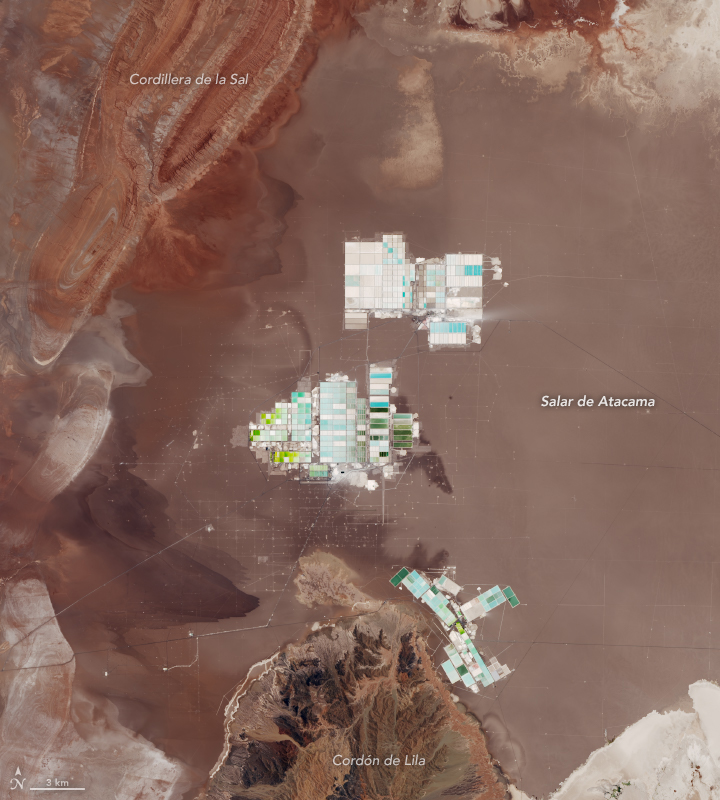
\includegraphics[width=0.48\linewidth]{images/book2/atacama-ponds.jpg}

{\small Lagoas de evaporação de salmoura de lítio no Salar de Atacama,
vistas da órbita (Landsat 8, 2018; NASA Earth Observatory, domínio
público, Wikimedia Commons). A cor de cada lagoa muda à medida que a
salmoura se concentra e os sais cristalizam.}
\end{omfigure}

\section{O hidrogênio e os hidretos}

O hidrogênio tem um elétron: pode perdê-lo (\ce{H+}, transportado pela
água como \ce{H3O+}), compartilhá-lo (\omterm{def:b1:lewis-resonance-vsepr:lewis}{ligações covalentes}) ou ganhar um
(\ce{H-}, com a \omterm{def:b1:quantum-numbers:configuration}{configuração eletrônica} do hélio). O que ele faz depende
de seu parceiro.

\begin{definition}[Hidretos]\label{def:b1:s-block:hydride}
Um \emph{hidreto}\index{hidreto} é um composto binário do hidrogênio com
outro elemento. Os \emph{hidretos salinos}\index{hidreto salino}, formados
com os \omterm{def:b1:s-block:families}{metais alcalinos} e os alcalinoterrosos mais pesados (\ce{LiH},
\ce{NaH}, \ce{CaH2}), são sólidos iônicos que contêm \ce{H-}. Os \emph{hidretos
covalentes}\index{hidreto covalente}, formados com os elementos do \omterm{def:b1:periodicity:table}{bloco} p
(\ce{CH4}, \ce{NH3}, \ce{H2O}, \ce{HCl}), são moleculares. Os \emph{hidretos
metálicos}\index{hidreto metalico@hidreto metálico}, formados com alguns metais de transição,
são sólidos em que o hidrogênio ocupa \omterm{def:b1:crystals-metals:site}{sítios intersticiais} do retículo
do metal, muitas vezes com composição variável.
\end{definition}

O íon \omterm{def:b1:s-block:hydride}{hidreto} é uma base e um \omterm{def:b1:nernst:couple}{redutor} muito fortes: os \omterm{def:b1:s-block:hydride}{hidretos salinos}
reagem com a água, \ce{NaH + H2O -> NaOH + H2}, e servem como agentes
secantes de solventes e como bases em síntese orgânica (\cref{ch:b1:alcohol-activation}).
Os \omterm{def:b1:s-block:hydride}{hidretos covalentes} do segundo \omterm{def:b1:periodicity:table}{período} mostram a tendência da
\omterm{def:b1:periodicity:electronegativity}{eletronegatividade} ao longo dele: \ce{CH4} nem ácido nem básico, \ce{NH3}
básico, \ce{H2O} anfótero, \ce{HF} ácido.

\section{Os metais alcalinos}

\begin{definition}[Metais alcalinos e alcalinoterrosos]\label{def:b1:s-block:families}
Os \emph{metais alcalinos}\index{metal alcalino} (Li, Na, K, Rb, Cs, Fr)
formam o \omterm{def:b1:periodicity:table}{grupo} 1, com um \omterm{def:b1:quantum-numbers:configuration}{elétron de valência} \textit{ns}$^1$; os
\emph{metais alcalinoterrosos}\index{metal alcalinoterroso} (Be, Mg, Ca, Sr,
Ba, Ra) formam o \omterm{def:b1:periodicity:table}{grupo} 2, com \textit{ns}$^2$. Seus elementos constituem
o \omterm{def:b1:periodicity:table}{bloco} s.
\end{definition}

\begin{proposition}[Os metais alcalinos são redutores fortes]\label{prop:b1:s-block:reducing-power}
Os \omterm{def:b1:s-block:families}{metais alcalinos} têm as menores \omterm{def:b1:periodicity:ionisation-energy}{primeiras energias de ionização} de
seus \omterm{def:b1:periodicity:table}{períodos} (Li \qty{5.39}{eV}, Na 5.14, K 4.34) e \omterm{def:b1:nernst:electrode-potential}{potenciais padrão}
muito negativos (\ce{Li+}/\ce{Li} $-3.04$~V, \ce{Na+}/\ce{Na} $-2.71$,
\ce{K+}/\ce{K} $-2.94$): eles reduzem a água e só são encontrados na
natureza como íons \ce{M+}.
\end{proposition}
% ledger: ie:Li, ie:Na, ie:K (E0 computed in figdata/bachelor-1/standard-potentials.py)

\begin{proof}
Um único elétron fora de um caroço de gás nobre, longe do núcleo e
blindado pelas camadas internas (\cref{ch:b1:periodicity}), é facilmente
removido. Em água, o pequeno íon \ce{M+} é fortemente hidratado, o que
torna o potencial do par ainda mais baixo. Com $E^\circ$ mais de
\qty{2.2}{V} abaixo da reta da água a pH 7 ($-0.41$~V), a reação
\ce{2M + 2H2O -> 2M+ + 2OH- + H2} tem uma constante enorme
(\cref{prop:b1:nernst:equilibrium-constant}).
\end{proof}

\begin{omfigure}
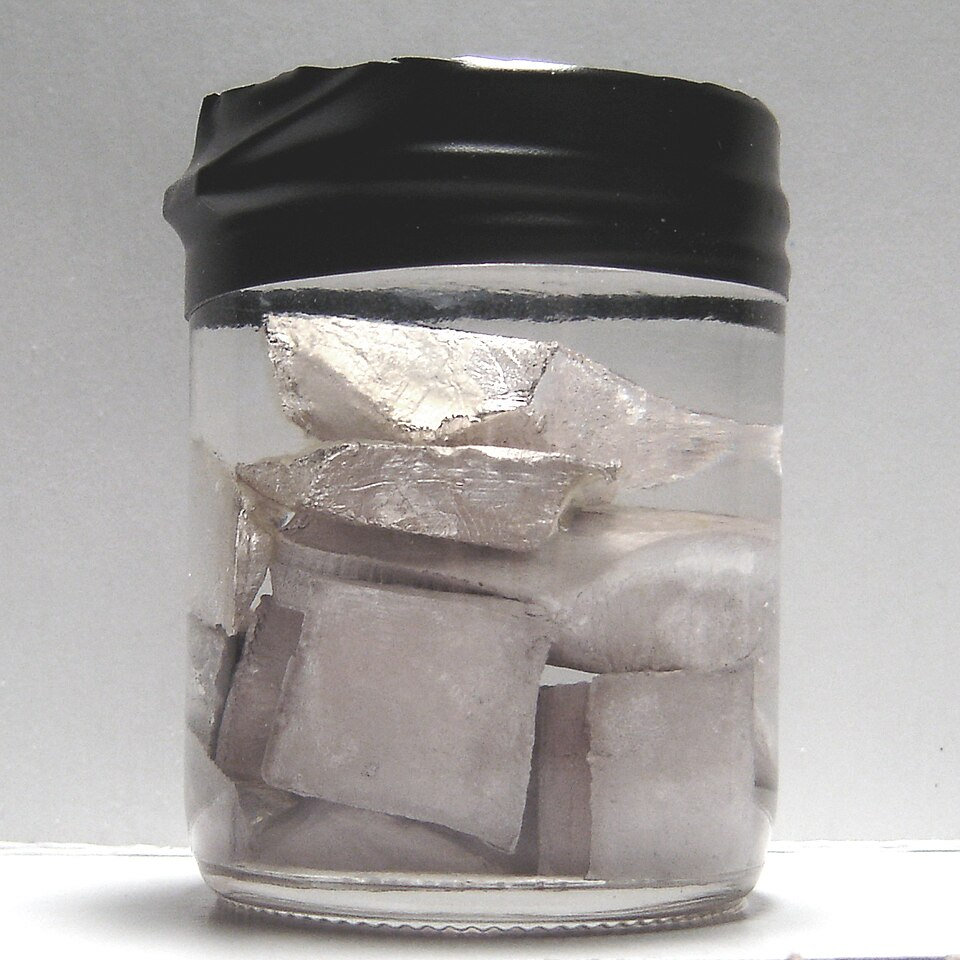
\includegraphics[height=4.6cm]{images/book2/sodium-oil.jpg}\hspace{0.8em}%
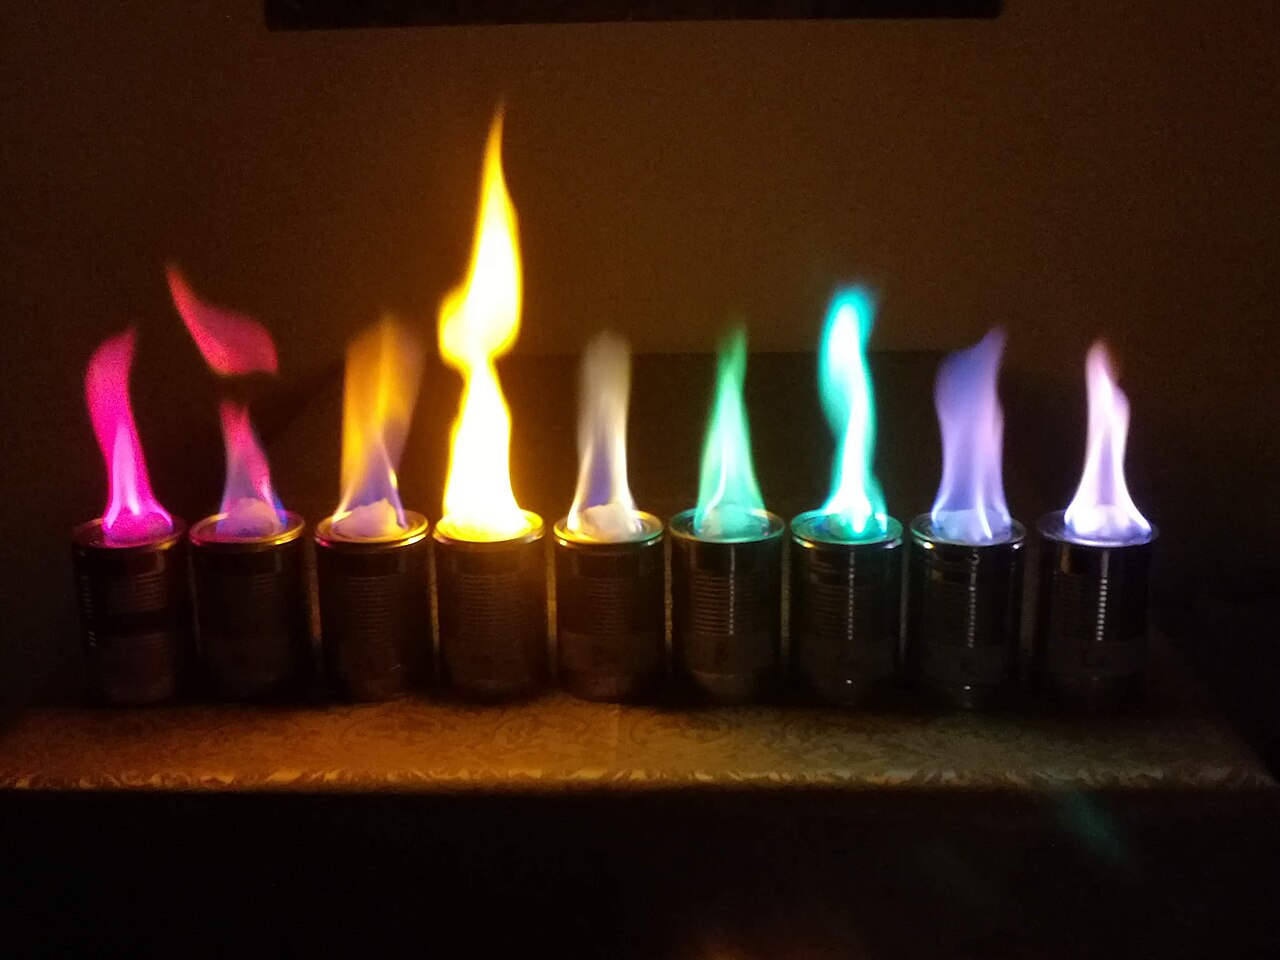
\includegraphics[height=4.6cm]{images/book2/flame-colours.jpg}

{\small À esquerda: o sódio é guardado sob óleo mineral, longe do ar e da
umidade (fotografia de Justin Urgitis, CC BY-SA 2.5). À direita: cores de
chama, da esquerda para a direita, de compostos de lítio, estrôncio,
cálcio, sódio, bário, boro, cobre, césio e potássio: os elétrons
excitados na chama voltam a níveis mais baixos emitindo luz em
comprimentos de onda característicos de cada elemento
(\cref{ch:b1:quantum-numbers}) (fotografia de Hegelrast, CC BY-SA 4.0).
Ambas da Wikimedia Commons.}
\end{omfigure}

\begin{inthelab}[Uma demonstração, não um experimento]
A reação do sódio com a água só é mostrada por um professor, atrás de uma
tela de proteção, com um pedaço do tamanho de uma lentilha jogado em uma
grande cuba de água contendo fenolftaleína: o metal funde em uma bolinha
que corre, o hidrogênio chia, e o rastro rosa mostra o hidróxido
formado. O potássio inflama o hidrogênio. Pedaços maiores explodem. O
sódio é cortado sob óleo, manipulado com pinça, e seus resíduos são
destruídos com etanol, nunca com água.
\end{inthelab}

O lítio é a exceção do seu grupo: o menor íon, o mais fortemente
hidratado, logo o potencial mais negativo, e no entanto o mais lento a
reagir com a água. Seus compostos se parecem com os do magnésio (o
carbonato e o fosfato de lítio são pouco solúveis, como os do magnésio),
uma relação diagonal na tabela periódica. Os \omterm{def:b1:s-block:families}{metais alcalinos} são
produzidos por eletrólise de seus cloretos fundidos, já que nenhum
\omterm{def:b1:nernst:couple}{redutor} químico é forte o bastante; as reações de eletrodo dessas células
são estudadas no volume do 2.º~ano.

\section{Os compostos de sódio na indústria}

\begin{definition}[Caráter dos óxidos]\label{def:b1:s-block:oxide-character}
Um \emph{óxido básico}\index{oxido basico@óxido básico} reage com a água
dando um hidróxido, ou com ácidos dando sais (\ce{Na2O}, \ce{CaO}); um
\emph{óxido ácido}\index{oxido acido@óxido ácido} reage com a água dando
um ácido, ou com bases dando sais (\ce{CO2}, \ce{SO3}, \ce{P4O10}); um
\emph{óxido anfótero}\index{oxido anfotero@óxido anfótero} reage tanto com
ácidos quanto com bases (\ce{Al2O3}, \ce{ZnO}). Ao longo de um \omterm{def:b1:periodicity:table}{período}, os
óxidos passam de básicos (metais, à esquerda) a ácidos (não metais, à direita).
\end{definition}

O hidróxido de sódio é produzido por eletrólise da salmoura (o processo
cloro-álcali, que também fornece cloro e hidrogênio). O carbonato de
sódio, ou barrilha, usado para vidro, detergentes e extração de lítio, é
extraído como o mineral trona ou produzido a partir de sal e calcário: em
2025 o mundo produziu cerca de 71 milhões de toneladas, 19 milhões de
jazidas naturais e 52 milhões sintéticos, a maior parte pelo processo Solvay.
% ledger: usgs:sodaash-total-2025, usgs:sodaash-natural-2025, usgs:sodaash-synthetic-2025

\begin{proposition}[O processo Solvay]\label{prop:b1:s-block:solvay}
O processo Solvay converte cloreto de sódio e carbonato de cálcio em
carbonato de sódio e cloreto de cálcio, \ce{2NaCl + CaCO3 -> Na2CO3 +
CaCl2}, por etapas em que a amônia e o dióxido de carbono são reciclados.
\end{proposition}

\begin{proof}
As etapas são: (1) \ce{CaCO3 -> CaO + CO2} (forno); (2) \ce{NaCl + NH3 +
CO2 + H2O -> NaHCO3 + NH4Cl} (carbonatação da salmoura amoniacal; o
hidrogenocarbonato, o sal menos solúvel presente, precipita); (3)
\ce{2NaHCO3 -> Na2CO3 + CO2 + H2O} (calcinação); (4) \ce{CaO + H2O ->
Ca(OH)2}; (5) \ce{Ca(OH)2 + 2NH4Cl -> CaCl2 + 2NH3 + 2H2O} (recuperação
da amônia). Somando $(1) + 2\times(2) + (3) + (4) + (5)$, \ce{NH3},
\ce{CO2}, \ce{NH4Cl}, \ce{NaHCO3}, \ce{CaO}, \ce{Ca(OH)2} e a água se cancelam:
\ce{2NaCl + CaCO3 -> Na2CO3 + CaCl2}.
\end{proof}

\begin{omfigure}
\begin{tikzpicture}[font=\small, >={Stealth}, box/.style={draw, rounded corners, fill=omDef!8, minimum width=2.6cm, minimum height=0.8cm, align=center}]
  \node[box] (kiln) at (0,0) {forno de cal\\\ce{CaCO3 -> CaO + CO2}};
  \node[box] (tower) at (5.3,0) {torre de carbonatação\\\ce{NaHCO3} precipita};
  \node[box] (calc) at (10.2,0) {calcinador\\\ce{NaHCO3} $\to$ \ce{Na2CO3}};
  \node[box] (slake) at (0,-2.6) {hidratador de cal\\\ce{CaO + H2O -> Ca(OH)2}};
  \node[box] (still) at (5.3,-2.6) {destilador de amônia\\\ce{NH4Cl + Ca(OH)2}};
  \draw[->, thick] (kiln) -- node[above] {\ce{CO2}} (tower);
  \draw[->, thick] (tower) -- node[above, font=\scriptsize] {\ce{NaHCO3}} (calc);
  \draw[->, thick] (calc.north) -- ++(0,0.6) -| node[pos=0.25, above] {\ce{CO2} reciclado} (tower.north);
  \draw[->, thick] (kiln) -- node[left] {\ce{CaO}} (slake);
  \draw[->, thick] (slake) -- node[above, font=\scriptsize] {\ce{Ca(OH)2}} (still);
  \draw[->, thick] (tower) -- node[right] {\ce{NH4Cl}} (still);
  \draw[->, thick] (still.east) -- ++(1.2,0) |- node[pos=0.25, right] {\ce{NH3} reciclada} ($(tower.east)+(0,-0.25)$);
  \draw[<-, thick] (tower.north west) -- ++(-0.5,0.6) node[above] {salmoura \ce{NaCl}};
  \draw[->, thick] (calc.east) -- ++(0.8,0) node[right] {\ce{Na2CO3}};
  \draw[->, thick] (still.south) -- ++(0,-0.6) node[below] {\ce{CaCl2}};
\end{tikzpicture}

{\small O processo Solvay. O dióxido de carbono e a amônia circulam em
ciclos; entram sal e calcário, saem barrilha e cloreto de cálcio.}
\end{omfigure}

\begin{omfigure}
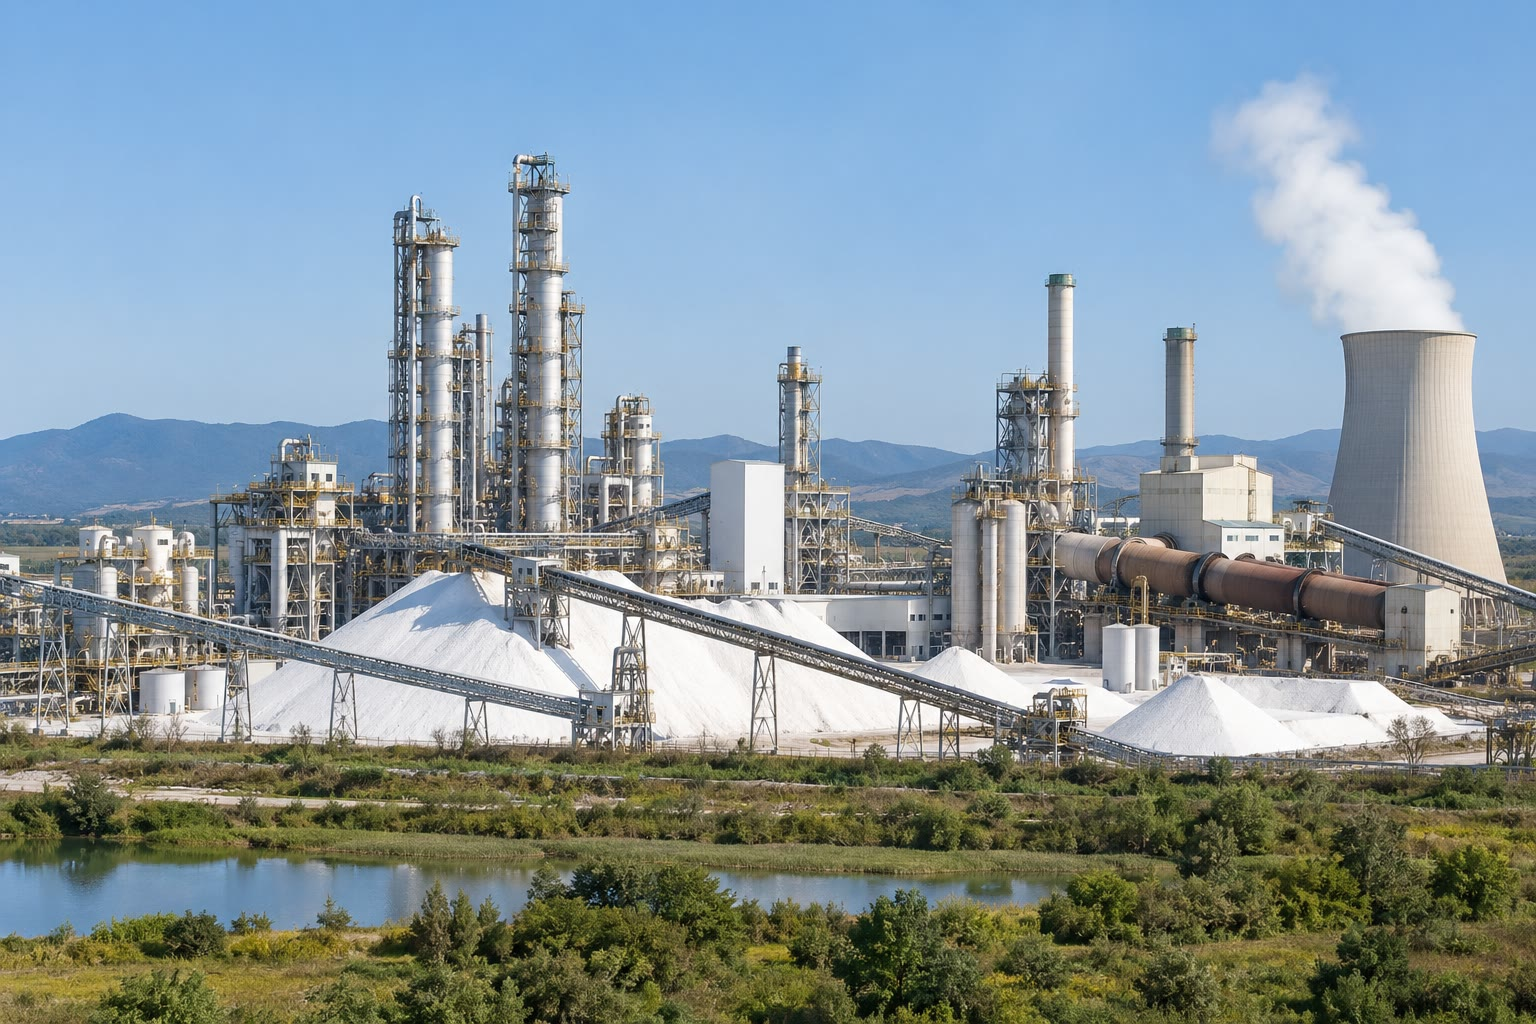
\includegraphics[width=0.55\linewidth]{images/book2/ai/b1-26-soda-ash-plant.jpg}

{\small Uma fábrica de barrilha: fornos de cal, torres de carbonatação e
pilhas de carbonato de sódio.}
\end{omfigure}

\begin{method}[Balanço de massa em um fluxograma]\label{met:b1:s-block:mass-balance}
\begin{enumerate}
  \item Escreva a equação global (soma das etapas, com as espécies
        recicladas canceladas).
  \item A partir do produto desejado, calcule as quantidades de
        matérias-primas com a equação global e depois corrija pelo
        \omterm{def:b1:extent-q-and-k:fractional-extent}{rendimento} de cada etapa.
  \item Para uma espécie reciclada, calcule apenas a reposição necessária
        para compensar suas perdas.
  \item Verifique o balanço de cada elemento entre entradas e saídas.
\end{enumerate}
\end{method}

\section{Os metais alcalinoterrosos}

O magnésio e o cálcio são menos reativos que os \omterm{def:b1:s-block:families}{metais alcalinos}
(energias de ionização maiores: Mg \qty{7.65}{eV}, Ca 6.11; dois elétrons
a perder), mas continuam sendo \omterm{def:b1:nernst:couple}{redutores} fortes ($E^\circ$ de \ce{Mg^2+}/\ce{Mg} $-2.36$~V).
O magnésio queima no ar com uma luz branca ofuscante; sua película de
óxido o protege à temperatura ambiente. O magnésio é recuperado da água
do mar precipitando seu hidróxido com cal, $\mathrm{p}K_s = 11.25$
(\cref{ch:b1:precipitation}).
% ledger: ie:Mg, ie:Ca

\begin{proposition}[O ciclo da cal]\label{prop:b1:s-block:lime-cycle}
Calcário, cal virgem, cal hidratada e de novo calcário formam um ciclo:
\ce{CaCO3 -> CaO + CO2} (aquecido em um forno); \ce{CaO + H2O -> Ca(OH)2}
(extinção, fortemente exotérmica); \ce{Ca(OH)2 + CO2 -> CaCO3 + H2O}
(endurecimento da argamassa de cal ao ar). O ciclo como um todo nada muda
quimicamente, mas armazena e libera energia e dióxido de carbono.
\end{proposition}

\begin{proof}
Somando as três equações, todas as espécies se cancelam. A decomposição
do carbonato exige calor, liberado de novo nas duas outras etapas; o
\ce{CO2} desprendido no forno é reabsorvido, lentamente, pela argamassa.
\end{proof}

\begin{omfigure}
\begin{tikzpicture}[font=\small, >={Stealth}]
  \node[draw, rounded corners, fill=omDef!8] (a) at (90:2.0) {\ce{CaCO3} calcário};
  \node[draw, rounded corners, fill=omDef!8] (b) at (-30:2.0) {\ce{CaO} cal virgem};
  \node[draw, rounded corners, fill=omDef!8] (c) at (210:2.0) {\ce{Ca(OH)2} cal hidratada};
  \draw[->, thick] (a) to[bend left=25] node[right, align=left] {calor\\$-\ce{CO2}$} (b);
  \draw[->, thick] (b) to[bend left=25] node[below] {$+\ce{H2O}$} (c);
  \draw[->, thick] (c) to[bend left=25] node[left, align=right] {$+\ce{CO2}$\\$-\ce{H2O}$} (a);
\end{tikzpicture}

{\small O ciclo da cal, do calcário à argamassa e de volta ao carbonato
de cálcio.}
\end{omfigure}

\section{O lítio}

\begin{omfigure}
\begin{tikzpicture}
\begin{axis}[
  xbar, width=0.78\linewidth, height=5.4cm, xmin=0, xmax=110,
  symbolic y coords={CA,ML,BR,AR,ZW,CL,CN,AU}, ytick=data,
  yticklabels={Canadá, Mali, Brasil, Argentina, Zimbábue, Chile, China, Austrália},
  xlabel={lítio extraído em 2025 (milhares de toneladas de Li, estimativas)}, bar width=8pt,
  nodes near coords, every node near coord/.append style={font=\scriptsize},
  tick label style={font=\small}, label style={font=\small}, enlarge y limits=0.1]
\addplot[fill=omDef!45, draw=omDef] coordinates {(5.6,CA) (9.4,ML) (12,BR) (23,AR) (28,ZW) (56,CL) (62,CN) (92,AU)};
\end{axis}
\end{tikzpicture}

{\small Os maiores produtores de lítio em 2025 (estimativas; total mundial
de cerca de \num{290000} toneladas de lítio). A Austrália explora rocha
dura (espodumênio); o Chile e a Argentina bombeiam salmouras.}
% ledger: usgs:li-canada-2025, usgs:li-mali-2025, usgs:li-brazil-2025, usgs:li-argentina-2025, usgs:li-zimbabwe-2025, usgs:li-chile-2025, usgs:li-china-2025, usgs:li-australia-2025, usgs:li-world-2025
\end{omfigure}

A salmoura é concentrada por evaporação, o magnésio é removido com cal,
e o carbonato de lítio é precipitado com barrilha. O carbonato de lítio
tem a propriedade incomum de ser menos solúvel a quente que a frio:
\qty{1.31}{\percent} em massa a \qty{20}{\celsius}, \qty{0.84}{\percent} a
\qty{80}{\celsius}, \qty{0.71}{\percent} a \qty{100}{\celsius}. Por isso ele
é precipitado a partir de solução quente, como calcula o problema de fim
de semana.
% ledger: sol:Li2CO3-20, sol:Li2CO3-80, sol:Li2CO3-100

\section{Exercícios}

\begin{exercise}[$\star$]\label{exo:b1:s-block:1}
Classifique como \omterm{def:b1:s-block:hydride}{hidreto salino}, covalente ou metálico: \ce{KH}, \ce{SiH4},
\ce{CaH2}, \ce{H2S}, \ce{PdH_{0.6}}. Escreva a reação de \ce{CaH2} com a água.
\end{exercise}

\begin{exercise}[$\star$]\label{exo:b1:s-block:2}
Escreva as reações do lítio, do sódio e do potássio com a água, e do
magnésio com ácido clorídrico diluído.
\end{exercise}

\begin{exercise}[$\star$]\label{exo:b1:s-block:3}
Classifique como básico, ácido ou anfótero: \ce{Na2O}, \ce{MgO}, \ce{Al2O3},
\ce{SiO2}, \ce{SO3}, \ce{ZnO}, \ce{CO2}. Escreva uma reação para cada tipo.
\end{exercise}

\begin{exercise}[$\star$]\label{exo:b1:s-block:4}
Calcule a constante de \ce{2Na + 2H2O -> 2Na+ + 2OH- + H2} a pH 14 a partir dos
\omterm{def:b1:nernst:electrode-potential}{potenciais padrão}.
\end{exercise}

\begin{exercise}[$\star\star$]\label{exo:b1:s-block:5}
Explique as cores de chama do lítio (vermelha) e do sódio (amarela) usando
os \omterm{def:b1:quantum-numbers:energy-level}{níveis de energia} dos átomos (\cref{ch:b1:quantum-numbers}). Qual é a
energia de um fóton amarelo a \qty{589}{nm}?
\end{exercise}

\begin{exercise}[$\star\star$]\label{exo:b1:s-block:6}
Calcule a massa de calcário (\ce{CaCO3} puro) e de cloreto de sódio
necessária para uma tonelada de barrilha pelo processo Solvay, com um
\omterm{def:b1:extent-q-and-k:fractional-extent}{rendimento} global de \qty{90}{\percent} em relação ao cloreto de sódio.
\end{exercise}

\begin{exercise}[$\star\star$]\label{exo:b1:s-block:7}
A água do mar contém cerca de \qty{1.3}{g/L} de magnésio (dado do
exercício). A partir de que pH o hidróxido de magnésio começa a
precipitar? Que massa de cal hidratada precipita o magnésio de \qty{1.0}{m^3}?
\end{exercise}

\begin{exercise}[$\star\star$]\label{exo:b1:s-block:8}
Por que o lítio reage mais lentamente com a água que o potássio, embora
seu \omterm{def:b1:nernst:electrode-potential}{potencial padrão} seja mais baixo? Distinga termodinâmica e cinética.
\end{exercise}

\begin{exercise}[$\star\star$]\label{exo:b1:s-block:9}
Calcule a massa de cal virgem obtida a partir de uma tonelada de calcário
e o volume de \ce{CO2} liberado, a \qty{25}{\celsius} e \qty{1}{bar}.
\end{exercise}

\begin{exercise}[$\star\star\star$]\label{exo:b1:s-block:10}
O mundo extraiu cerca de \num{290000} toneladas de lítio em 2025. A que
massa de carbonato de lítio isso corresponde? Se uma bateria de carro
contém \qty{8}{kg} de lítio (dado do exercício), quantas baterias isso
poderia abastecer?
\end{exercise}

\begin{exercise}[$\star\star\star$]\label{exo:b1:s-block:11}
Mostre, a partir dos dados do capítulo, que a \omterm{def:b1:precipitation:solubility}{solubilidade} do carbonato de
lítio diminui com a temperatura, e explique por que precipitá-lo a quente
melhora a recuperação a partir de uma salmoura.
\end{exercise}

\begin{exercise}[$\star\star\star$]\label{exo:b1:s-block:12}
Na etapa (2) do processo Solvay, a solução contém \ce{Na+},
\ce{NH4+}, \ce{Cl-} e \ce{HCO3-}. Explique por que precipita o
hidrogenocarbonato de sódio e não o cloreto de amônio, e por que o
processo precisa de amônia e não de hidróxido de sódio.
\end{exercise}

\section{Problema: lítio a partir da salmoura}

\begin{problem}[{Problema de fim de semana --- concentrar uma salmoura de
lítio, remover o magnésio com cal, precipitar o carbonato de lítio com
barrilha, e a massa de carbonato de lítio recuperada de um metro cúbico}]
\label{pb:b1:s-block:1}
Uma salmoura bombeada de debaixo de um salar contém \qty{1.5}{g/L} de
lítio e \qty{0.60}{g/L} de magnésio (como íons, com muito cloreto de
sódio). A evaporação em lagoas a concentra quatro vezes. Um metro cúbico
da salmoura concentrada é então tratado: a cal remove o magnésio, a
barrilha o cálcio, e a barrilha a quente precipita por fim o carbonato de
lítio a \qty{80}{\celsius}. Dados: massas molares (\unit{g/mol}) Li 6.9, Mg 24.3,
\ce{Ca(OH)2} 74.1, \ce{Na2CO3} 106.0, \ce{Li2CO3} 73.8; $\mathrm{p}K_s$
\ce{Mg(OH)2} 11.25, \ce{CaCO3} 8.30; $\mathrm{p}K_e = 14.00$; \omterm{def:b1:precipitation:solubility}{solubilidade}
do \ce{Li2CO3} \qty{0.84}{\percent} em massa a \qty{80}{\celsius}; tome
o licor final como \qty{1.00}{m^3} de massa específica \qty{1.0}{kg/L}.

\medskip
\noindent\textbf{Parte I --- A concentração.}
\begin{enumerate}
  \item Calcule as concentrações de lítio e de magnésio na salmoura
        concentrada.
  \item Que volume de água evapora por metro cúbico de salmoura
        concentrada?
  \item Por que se usa a evaporação solar e não o aquecimento?
  \item Que sal cristaliza primeiro nas lagoas, e por quê?
  \item Calcule as quantidades de matéria de lítio e de magnésio em um metro cúbico.
  \item Por que o magnésio precisa ser removido antes de o lítio ser precipitado?
\end{enumerate}

\medskip
\noindent\textbf{Parte II --- A remoção do magnésio e do cálcio.}
\begin{enumerate}[resume]
  \item Escreva a reação dos íons magnésio com a cal hidratada.
  \item Calcule a massa de cal hidratada necessária (estequiométrica).
  \item A que pH \qty{99.9}{\percent} do magnésio está precipitado?
  \item Por que o lítio não é precipitado como hidróxido?
  \item Escreva a remoção do cálcio introduzido, com barrilha.
  \item Calcule a massa de barrilha necessária para essa etapa.
\end{enumerate}

\medskip
\noindent\textbf{Parte III --- O carbonato de lítio.}
\begin{enumerate}[resume]
  \item Escreva a precipitação do carbonato de lítio.
  \item Calcule a massa de barrilha necessária para o lítio.
  \item Calcule a massa teórica de carbonato de lítio.
  \item Por que a precipitação é feita a \qty{80}{\celsius}?
  \item Que massa de carbonato de lítio fica dissolvida no licor?
  \item Como o precipitado é lavado sem perder muito dele?
\end{enumerate}

\medskip
\noindent\textbf{Parte IV --- Balanço.}
\begin{enumerate}[resume]
  \item Calcule a massa de carbonato de lítio recuperada.
  \item Calcule a taxa de recuperação do lítio.
  \item Sugira o que se faz com o licor.
  \item Compare o lítio de um metro cúbico com a produção mundial de
        2025: quantos metros cúbicos essa produção representaria?
  \item Indique a massa de carbonato de lítio recuperada por metro cúbico
        de salmoura concentrada.
\end{enumerate}
\end{problem}
